\documentclass[sans,mathserif]{beamer}
\setbeamersize{text margin left=4mm,text margin right=4mm} 
%%%%%%%%%%%% 
\mode<presentation>
{
  \usetheme{default}      % or try AnnArbor, Boadilla, Darmstadt, Madrid, Warsaw, EastLansing 
  \usecolortheme{default} % or try albatross, beaver, crane, ...
  \usefonttheme{serif}  % or try serif, structurebold, professionalfonts, ...
  \setbeamertemplate{navigation symbols}{}
  \setbeamertemplate{caption}[numbered]
} 
%%%%%%%%%%%% 
\usepackage{kotex}
\usepackage{tcolorbox}
\usepackage{xcolor}
\usepackage{bbm}
\usepackage{txfonts}
\usepackage{enumerate}
\usepackage{tikz}
\usepackage{calc}
\usepackage{accents}
\usepackage{tcolorbox}
\usepackage{enumitem}
% \usepackage{commath}
\usepackage{hyperref}
\usepackage{textcomp}
\usepackage{amsmath}
% \usepackage{mathtools}
\usepackage{hyperref}
\usepackage{minted}
\hypersetup{
    colorlinks=true,
    linkcolor=blue,
    filecolor=magenta,      
    urlcolor=cyan,
    pdftitle={Overleaf Example},
    pdfpagemode=FullScreen,
    }

\urlstyle{same}
\setlist[itemize,1]{label=\textopenbullet}
\setlist[itemize,2]{label=$\diamond$}
\setlist[itemize,3]{label=$\cdot$}
\usepackage{ulem}
\renewcommand<>{\sout}[1]{\alt#2{\beameroriginal{\sout}{#1}}{#1}}
%%%%%%%%%%%% 
\AtBeginSection[]
{
     \begin{frame}
		\frametitle{Outline}
%		\hypersetup{linkcolor=dgreen}
		\hypersetup{linkcolor=.}
%		\fontsize{10pt}{8pt}\selectfont
		% \scriptsize
%		\tableofcontents[currentsection,subsectionstyle=hide]
		\tableofcontents[currentsection,subsectionstyle=show/shaded]
		\small
%     \addtocounter{framenumber}{-1}
		\end{frame}
} 
%%%%%%%%%%%% 
% \AtBeginSubsection[]
% {
% 		\begin{frame}
% 		\frametitle{Outline}
% 		\hypersetup{linkcolor=.}
% 		\scriptsize
% 		\tableofcontents[currentsection,currentsubsection]
%      %     \addtocounter{framenumber}{-1}
% 		\end{frame}
% } 
%%%% Definition of Color %%%%%%%% 
\definecolor{dred}{RGB}{220,26,27}
\definecolor{dgreen}{RGB}{150,252,150}
\definecolor{dyellow}{RGB}{254,226,3}
\definecolor{dblue}{RGB}{102,102,255}
\definecolor{dbrown}{RGB}{155,123,49}
%%%% Headline %%%%%%%% 
\setbeamercolor{mycolor1}{fg=dblue,bg=dgreen}
\setbeamercolor{mycolor2}{fg=dgreen,bg=dblue}
\setbeamertemplate{headline}
{%
  \hbox{%
  \begin{beamercolorbox}[wd=.5\paperwidth,ht=2.5ex,dp=1.125ex]{mycolor1}%
		\hypersetup{linkcolor=.}
    \hbox to .5\paperwidth{\hfil\insertsectionhead\hfil}
  \end{beamercolorbox}%
  \begin{beamercolorbox}[wd=.5\paperwidth,ht=2.5ex,dp=1.125ex]{mycolor2}%
  		\hypersetup{linkcolor=.}
    \hbox to .5\paperwidth{\hfil\insertsubsectionhead\hfil}
  \end{beamercolorbox}}%
}
%%%%% Footline %%%%%%% 
\setbeamertemplate{footline}
{%
    \hbox{%
    \begin{beamercolorbox}[wd=\paperwidth,ht=3ex,dp=1.5ex,leftskip=2ex,rightskip=2ex]{mycolor1}
		\hypersetup{linkcolor=.}
		\usebeamerfont{title in head/foot}%
		% \insertsection \hfill
		\insertshorttitle \hfill
		\insertframenumber{} / \inserttotalframenumber
    \end{beamercolorbox}}%
}
%%%%%%%%%%%% 
% \DeclarePairedDelimiter\ceil{\lceil}{\rceil}
% \DeclarePairedDelimiter\floor{\lfloor}{\rfloor}
%\newcommand{\norm}[1]{\left\lVert#1\right\rVert}
%%%%%%%%%%%% 
\newcommand{\dbtilde}[1]{\accentset{\approx}{#1}}
\newcommand{\vardbtilde}[1]{\tilde{\raisebox{0pt}[0.95\height]{$\tilde{#1}$}}}
\newcommand{\tib}[1]{\textit{\textbf{#1}}}
%%%%%%%%%%%% 
\newcommand{\wine}[1]{\textcolor{dred}{#1}}
\newcommand{\water}[1]{\textcolor{dblue}{#1}}
\newcommand{\soop}[1]{\textcolor{dgreen}{#1}}
\newcommand{\rbc}[1]{\textcolor{blue}{#1}}
\newcommand{\mycirc}[1]{\raisebox{.5pt}{\textcircled{\raisebox{-.9pt} {#1}}}}
%%%%% Reference %%%%%
\makeatletter
%\renewcommand{\@makefnmark}{\makebox{[{\color{blue}\@thefnmark}]}}
%\renewcommand{\footnoterule}{\kern -3pt \moveright4mm\vbox{\hrule width 5cm height 0.3pt} \kern 2pt}
%\renewcommand\@makefntext[1]{\tiny{\color{red}\@thefnmark}\enspace #1}
\renewcommand\thefootnote{\textcolor{red}{\arabic{footnote}}}
\makeatother
\usepackage{filecontents}
\usepackage[style=phys, uniquename=false, maxbibnames=99, maxcitenames=2, backend=biber]{biblatex}
\addbibresource{Beamer.bib}
\setlength{\footnotesep}{2mm}
% \newcommand{\myref}[1]{\citeauthor{#1}\cite{#1}
\newcommand{\myref}[1]{\cite{#1}
  \let\thefootnote\relax
	\footnotetext{\tiny\hskip -0.5em\cite{#1}\enspace\fullcite{#1}}
	\let\thefootnote\svthefootnote}
\newcommand{\mycite}[1]{\citeauthor{#1}\cite{#1}}
\AtBeginEnvironment{frame}{\setcounter{footnote}{0}}
\renewcommand\multicitedelim{\addsemicolon\space}
\hypersetup{colorlinks,citecolor=blue,linkcolor=blue}
%%%%%%%%%%%%
%\defbibentryset{set:benn1}{benn1993,benn1992}
%\defbibentryset{set:ivan1}{ivan1987,diek1988,pere1988}
%%%%%%%%%%%% 
\setbeamercolor{title}{fg=dblue,bg=dgreen}
\title[%
2022 서울 국제 스마트팩토리 컨퍼런스\\ \& 액스포 참가 보고서(기술 파트)
]{%
\large 
2022 서울 국제 스마트팩토리 컨퍼런스\\ \& 액스포 참가 보고서(기술 파트)
}%
\author[J.H. Kim]{
김 지 환
}
\institute{스칼라웍스 선행기술팀}
%\logo{%
%  \makebox[0.95\paperwidth]{%
%    \hfill%
%    \includegraphics[width=3cm,keepaspectratio]{logo.jpg}%
%  }%
%}
{\tiny \date{{ Updated \today}}}
\begin{document}
%%%%%%%%%%%%%%%%%%%

\begin{frame}
  \titlepage
  %Speaker: {\bf Name}\\[1mm] 
  %\footnotesize 
  %Department of Applied , University,\\[1mm]
  %O-si, O-do, Republic of (South) Korea
\end{frame}
%%%%%%%%%%%%%%%%%%%
\logo{}
\usebackgroundtemplate{
  \parbox[c][\paperheight][c]{\paperwidth}
  {\centering\tikz\node[opacity=0.15]{
\includegraphics[scale=0.4]{bg.png}};}
}
%%%%%%%%%%%%%%%%%%%
\small
%%%%%%%%%%%%%%%%%%%
\begin{frame}
	{참관내용 요약}
	\begin{itemize}
		{\scriptsize
			\item {\bf일시}: 2022년 6월 24일 금요일 오전 9시 부터 17시까지.
			\vskip 3mm
			\item[\textbullet] {\bf장소}: 코엑스 서울 코엑스 그랜드볼룸(1F).
			\vskip 3mm
			\item {\bf참가자}: 김지환 선임, 신수민 대리.
			\vskip 3mm
			\item[\textbullet] {\bf참관내용}:
			\vskip 1mm
			(1)	참여기업의 전시 참관
			\vskip 1mm
			(2) 네 개의 강연 청강.
			\vskip 1mm

		}
	\end{itemize}
\end{frame}
%%%%%%%%%%%%%%%%%%%
\section{I. 방문 부스 및 기술 소개}
%%%%%%%%%%%%%%%%%%%
\subsection{TobiiPro}

\begin{frame}
  { TobiiPro}
  % \vskip 3mm
  
  \begin{itemize}
    {\scriptsize
    \item {\bf소비자의 잠재의식 분석에 활용}: 
    \vskip 1mm
	어떤 패키지 디자인이 효과적인지,
	\vskip 1mm
	소비자를 매장으로 끌어들이는 디스플레이는 무엇인지,
	\vskip 1mm
	매장 내 쇼핑 패턴과 제품 광고에 대한 관심도 파악,
	\vskip 1mm
	무엇이 구매를 포기하게 했는지,
	\vskip 1mm
	웹 사이트, 앱 및 소프트웨어 사용성을 점검 개선.
    \vskip 3mm
    \item[\textbullet] {\bf작업 현장의 효율성과 생산성을 향상시키고 안전성을 개선}
    \vskip 1mm
	숙련 직원의 노하우 매뉴얼화하여 신입 교육에 활용,
    \vskip 1mm
    인적 오류의 위험도 파악, 사고 예방 예측 모델 개발,
    \vskip 1mm
    작업환경 최적화 파악 및 재설계.
    } 
  \end{itemize}
  \begin{figure}
	\centering
	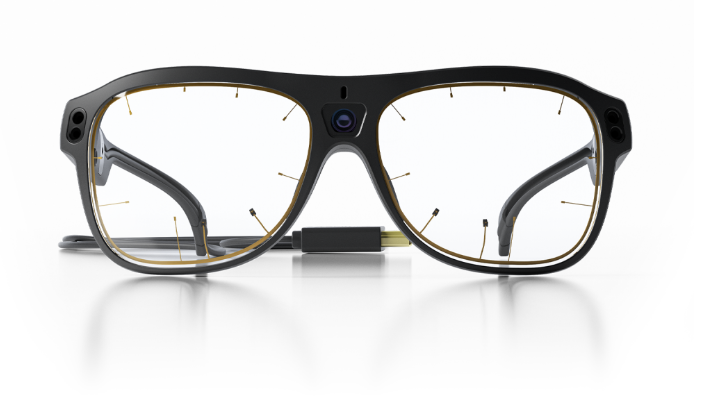
\includegraphics[width=0.25\textwidth]{./figures/tobiipro.png}
  \end{figure}
\end{frame}
%%%%%%%%%%%%%%%%%%%
\subsection{SIZL}

\begin{frame}
  {SIZL}
  % \vskip 3mm
  
  \begin{itemize}
    {\scriptsize
    \item[\textbullet] 고객사 기존 설비의 smart화 
    \item 독자 개발된 IoT 모듈 사용, 현장 설치 서버를 통해 빠른 데이터 수집
    \item[\textbullet] 전용 컨트롤러로 데이터를 직접 수집하여 처리 분석 가능
    \item Manufacturing Execution System (MES)는 생산 최적화를 위한 정보 제공 시스템
    \item Press Monitoring System (PMS) 기존 보유 프레스와 IoT 디바이스를 연동하여 오작동 이벤트 발생시 알람 제공 안정적인 생산 운영을 도움
    \item Welding Monitoring System (WMS) 용접기계에 IoT 센서 부착 실시간으로 상태와 생산량 등을 제공
    } 
  \end{itemize}
\end{frame}
%%%%%%%%%%%%%%%%%%%
\begin{frame}
	{SIZL}
	% \vskip 3mm
	
	\begin{itemize}
	  {\scriptsize

	  \item CNS Monitoring System (CMS) 절삭공구의 상태 생산량 모니터링 설비 이력이나 교환 주기 관리
	  \item Utilities Monitoring System (UMS) 공기압, 냉각수, 가스, 전략에 대한 정보 실시간 모니터링
	  \item Data Management System (DMS) 시즐 솔루션의 데이터를 중앙에서 관리 분석, 관리
	  } 
	\end{itemize}
	\begin{figure}
	  \centering
	  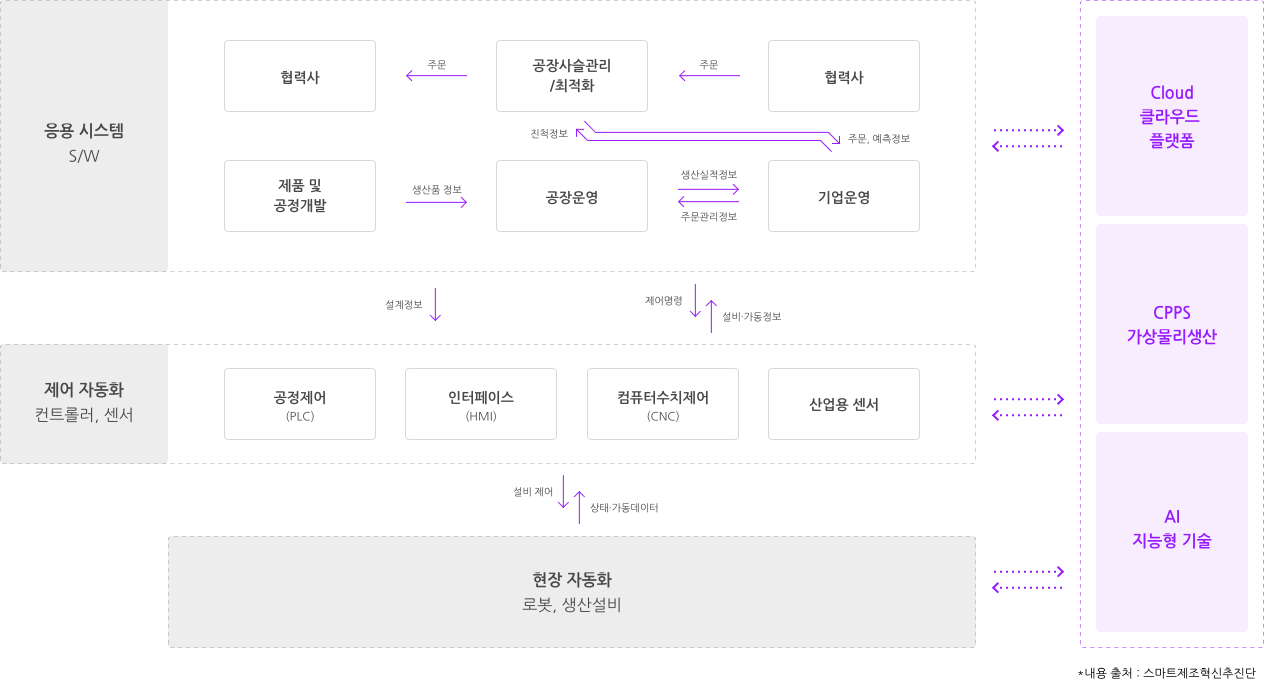
\includegraphics[width=0.7\textwidth]{./figures/sizl.png}
	\end{figure}
  \end{frame}
%%%%%%%%%%%%%%%%%%%
\subsection{TWiM}
\begin{frame}
	{TWiM}
	\begin{itemize}
	  {\scriptsize
	  \item 인공지능 검사장비와 룰에 기반한 하이브리드 비전 시스템으로 각 공정에 특화한 머신비전 표준화, 제조부터 출하까지 스마트팩토리를 위한 모든 솔루션 제공
	  \item T-MEGA: 제품 특성에따라 카메라 조명이 다양한 솔루션으로 적용 가능
	   검사 사양에 따른 맞춤형 광학기기 이용 다양한 결함 검사 가능
	   맞춤 개발로 어떤 부품 사이즈도 검사 가능
	   멀티스레드 처리를 통한 검사 구현 가능
	   불량의 한도 설정으로 수율 조정 가능
	  \item T-MES: 기존 MES 즉 생산관리, 자재관리, 모니터링은 물론 제조 현장에서 발생하는 데이터를 실시간으로 수집하여 통계적 분석 방식과 AI 분석 방식을 통해 설비가 최상의 상태로 유지되는 설비 분석 시스템이 추가된 차세대 설비 분석 시스템
	  \item 셀 폴딩기 검사: 제품당 16~20회 (초당 3.5회) 조건 이미지를 촬영 및 검사 진행, 분리막 찢김, 찍힘, 접힘, 이물 자국등의 표면 검사 시스템. Area Camera를 활용한 분리막 표면 검사
	  \item 2차전지 검사 시스템: Area Camera를 활용한 분리막의 이음새, 표면 검사, Line Scan Camera를 활용한 측면 스크래치, 이물 표면 검사 가능 (원통형 형상 자재 생산에 대한 확장 가능)
	  \item Alignment 비전 시스템 : 비정형 자재에 대한 특징 추츨 및 얼라인 가능
	  } 
	\end{itemize}
  \end{frame}
%%%%%%%%%%%%%%%%%%%
\subsection{NEUROCLE}
\begin{frame}
	{NEUROCLE}
	\begin{itemize}
	  {\scriptsize
	  \item 손쉽게 딥러닝 비전 기술 적용. 이미지 및 영상을 해석하기 쉬운 소프트웨어 연구 개발.
	  \item 데이터 관리, 모델링 뿐아니라 결과 분석까지 필요한 과정을 클릭 몇 번으로 자동화.
	  \item GUI 기반의 Trainer제공.
	  } 
	\end{itemize}
  \end{frame}
%%%%%%%%%%%%%%%%%%%
\section{II. 강연의 주요내용 요약}
\subsection{스마트 제조 혁신의 방향}
\begin{frame}
	{스마트 제조 혁신의 방향}
	\begin{itemize}
	  {\scriptsize
	  \item {\bf스마트 팩토리 발전 방향}
		\vskip 1mm
		다품종 소량 생산
		\vskip 1mm
		인간 로봇 협업
		\vskip 1mm
		메타버스 기반의 가상 공장
		\vskip 1mm
		숙련 경험 모사형 제조
		\vskip 1mm
		지능형 물류 시스템
		\vskip 1mm
		안전/예지 보전 시스템
	  
	  } 
	\end{itemize}
  \end{frame}
%%%%%%%%%%%%%%%%%%%
\begin{frame}
	{스마트 제조 혁신의 방향}
	\begin{itemize}
	  {\scriptsize
	  \item {\bf머신비전 시장에서 인공지능 기술 발전 방향}
		\vskip 1mm
		Edge AI: 온디바이스 AI를 위한 모델 경량화
		\vskip 1mm
		XAI: 판단 이유를 설명할 수 있는 AI
		\vskip 1mm
		Self Supervised Learning: 데이터 라벨링의 한계를 극복
		\vskip 1mm
		AboutML: 비효율적인 모델 개발 작업은 AI 활용.
		\vskip 1mm
		Generative AI: 데이터 증장 분야에도 활용
		\vskip 1mm
		Transfer learning: 사전에 학습된 모델을 활용
	  
	  } 
	\end{itemize}
  \end{frame}
%%%%%%%%%%%%%%%%%%%
\subsection{인공지능을 활용한 제조 혁신 방안}
\begin{frame}
	{인공지능을 활용한 제조 혁신 방안}
	\begin{itemize}
	  {\scriptsize
	  \item {\bf 인공지능 신뢰성의 필요성}
		\vskip 1mm
		우버 자율주행차 보행자 사망사고 원인 파악 필요.
		\vskip 1mm
		설명을 요구할 권리 - 알고리즘에 의해 행해진 결정에 대해 질문하고, 결정에 관여한 논리에 대해 의미있는 설명을 요구할 권리 EU의 일장 정보보호규정(GDPR)
		\vskip 1mm
		고위험 AI(자율주행, 생체신호, 신용정보, 인사평가)는 벌금이 6\%로 상향 예정
	\item {\bf설명가능 인공지능의 필요성}
		\vskip 1mm
		생성 모델의 내부를 분석하고 수정할 수 있음
		\vskip 1mm
		자율주행 딥러닝을 설명 가능
		\vskip 1mm
		우리 공장은 경쟁사에 비해 최적으로 운영되고 있을까?
		\vskip 1mm
		\href{https://drive.google.com/file/d/1VtFGSQ6uvlT3lQuPl4p60_XgLV_w09MH/view?usp=sharing}{\beamergotobutton{Link}}
	  } 
	\end{itemize}
  \end{frame}
%%%%%%%%%%%%%%%%%%%
\subsection{XR 기술을 활용한 Smart Factory 솔루션}
\begin{frame}
	{XR 기술을 활용한 Smart Factory 솔루션}
	\begin{itemize}
	  {\scriptsize
	  \item {\bf 문제를 해결하기 위한 현설적인 XR 솔루션 개발}
		\vskip 1mm
		빠르고 정확한 현장 파악, 문제 대응력 향상, 사고비용 감소 및 의사 결정 시간 단축
		\vskip 1mm
		작업 절차와 설비도면, 운전 데이터등 정보 증강, 업무 이해도 증가 및 업무 효율성 향상
		\vskip 1mm
		작업 안전 체크리스트 위험 구역 안내 등 안전 정보 증강, 안전관리 강화 및 안전사고 감소
	\item {\bf산업용 XR 솔루션}
		\vskip 1mm
		AR SW 개발 Toolkit(자체 개발 엔진, AR SDK)
		\vskip 1mm
		XR 특화 서버 서비스: 인증/보안, 연결, 관리, 부하 분산
		\vskip 1mm
		통합관리 콘솔: 멤버, 권한, 라이선스, 콘텐츠, 작업 관리 작업 진행률, 작업 보고 확인
		\vskip 1mm
		XR 기반 다자간 원격 협업: 원격에서 현장을 신속하고 정확하게 파악, XR가이드를 통해 업무지시 가능
		\vskip 1mm
		XR 콘텐츠 제작 및 뷰어: 노코드 방식으로 쉽고 빠르게 콘텐츠 제작, 배포, 수정 가능
		\vskip 1mm
		3D 현장 모니터링: 산업 현장을 3차원으로 디지털화, 현황 모니터링.
		
	  } 
	\end{itemize}
  \end{frame}
%%%%%%%%%%%%%%%%%%%

\section{III. 결론}
  \begin{frame}[fragile]
	{결론}
	  \scriptsize
	\begin{itemize}
		\item 공장 자동화 기업들은 \underline{MES를 차별화 하기 위한 기술 개발에 집중}하고 있음.
		\vskip 3mm
		\item 인공지능과 비전을 이용한 검사장비 업체들은 \underline{다양한 상황에서 적용 가능한 노하우를 누적하고 자체 응용프로그램을 개발} 하였음. 특히 \underline{고 해상도 이미지의 처리는 crop하여 처리하는 방식을 채택}하고 있음.
		\vskip 3mm
		\item \underline{XR의 좌표 설정에 있어 QR코드를 활용}하는 방법을 배우고 \underline{설명가능한 인공지능의 필요성}을 배울 수 있었음.
	\end{itemize}
  \end{frame}

%%%% Reference %%%%
\begin{filecontents}[nosearch]{Beamer.bib}
@ARTICLE{zhang,
  author={Zhang, Z.},
  journal={IEEE Transactions on Pattern Analysis and Machine Intelligence}, 
  title={A flexible new technique for camera calibration}, 
  year={2000},
  volume={22},
  number={11},
  pages={1330-1334},
  doi={10.1109/34.888718}
  }
% @ARTICLE{gabriele,
%   author={G. Galfre, A. Cardone F. Sandrelli},
%   title={3D Model Reconstruction from Stereo 2D Images}, 
%   url={https://github.com/ArtyZiff35/3D_Reconstruction_From_Stereo_Images/blob/master/documentation/3D_Model_Reconstruction_from_Stereo_2D_Images.pdf}
%   year={2018},
%   }
 
\end{filecontents}
%%%%%%%%%%%%%%%%%%%
\end{document}
